\section{Introduction}
\label{sec:intro}

The core objective for video understanding lies in mastering spatiotemporal representations, 
which inherently presents two formidable challenges: 
the large spatiotemporal redundancy within short video clips,
and the complex spatiotemporal dependencies among long contexts.
Although the once-dominant 3D convolutional neural networks (CNNs)\cite{c3d,i3d,slowfast} and video transformers\cite{timesformer,vivit}, 
effectively tackle one of the challenges mentioned by leveraging either local convolution or long-range attention, 
they fall short in addressing both simultaneously.
UniFormer~\cite{uniformer} attempts to integrate the advantages of both methods, 
but it struggles with modeling long videos,
which has been the major trend in recent research on video understanding~\cite{gemini,lwm} and generation~\cite{sora,vlogger}.


\begin{figure}[t]
    \centering
    \vspace{-0.3cm}
    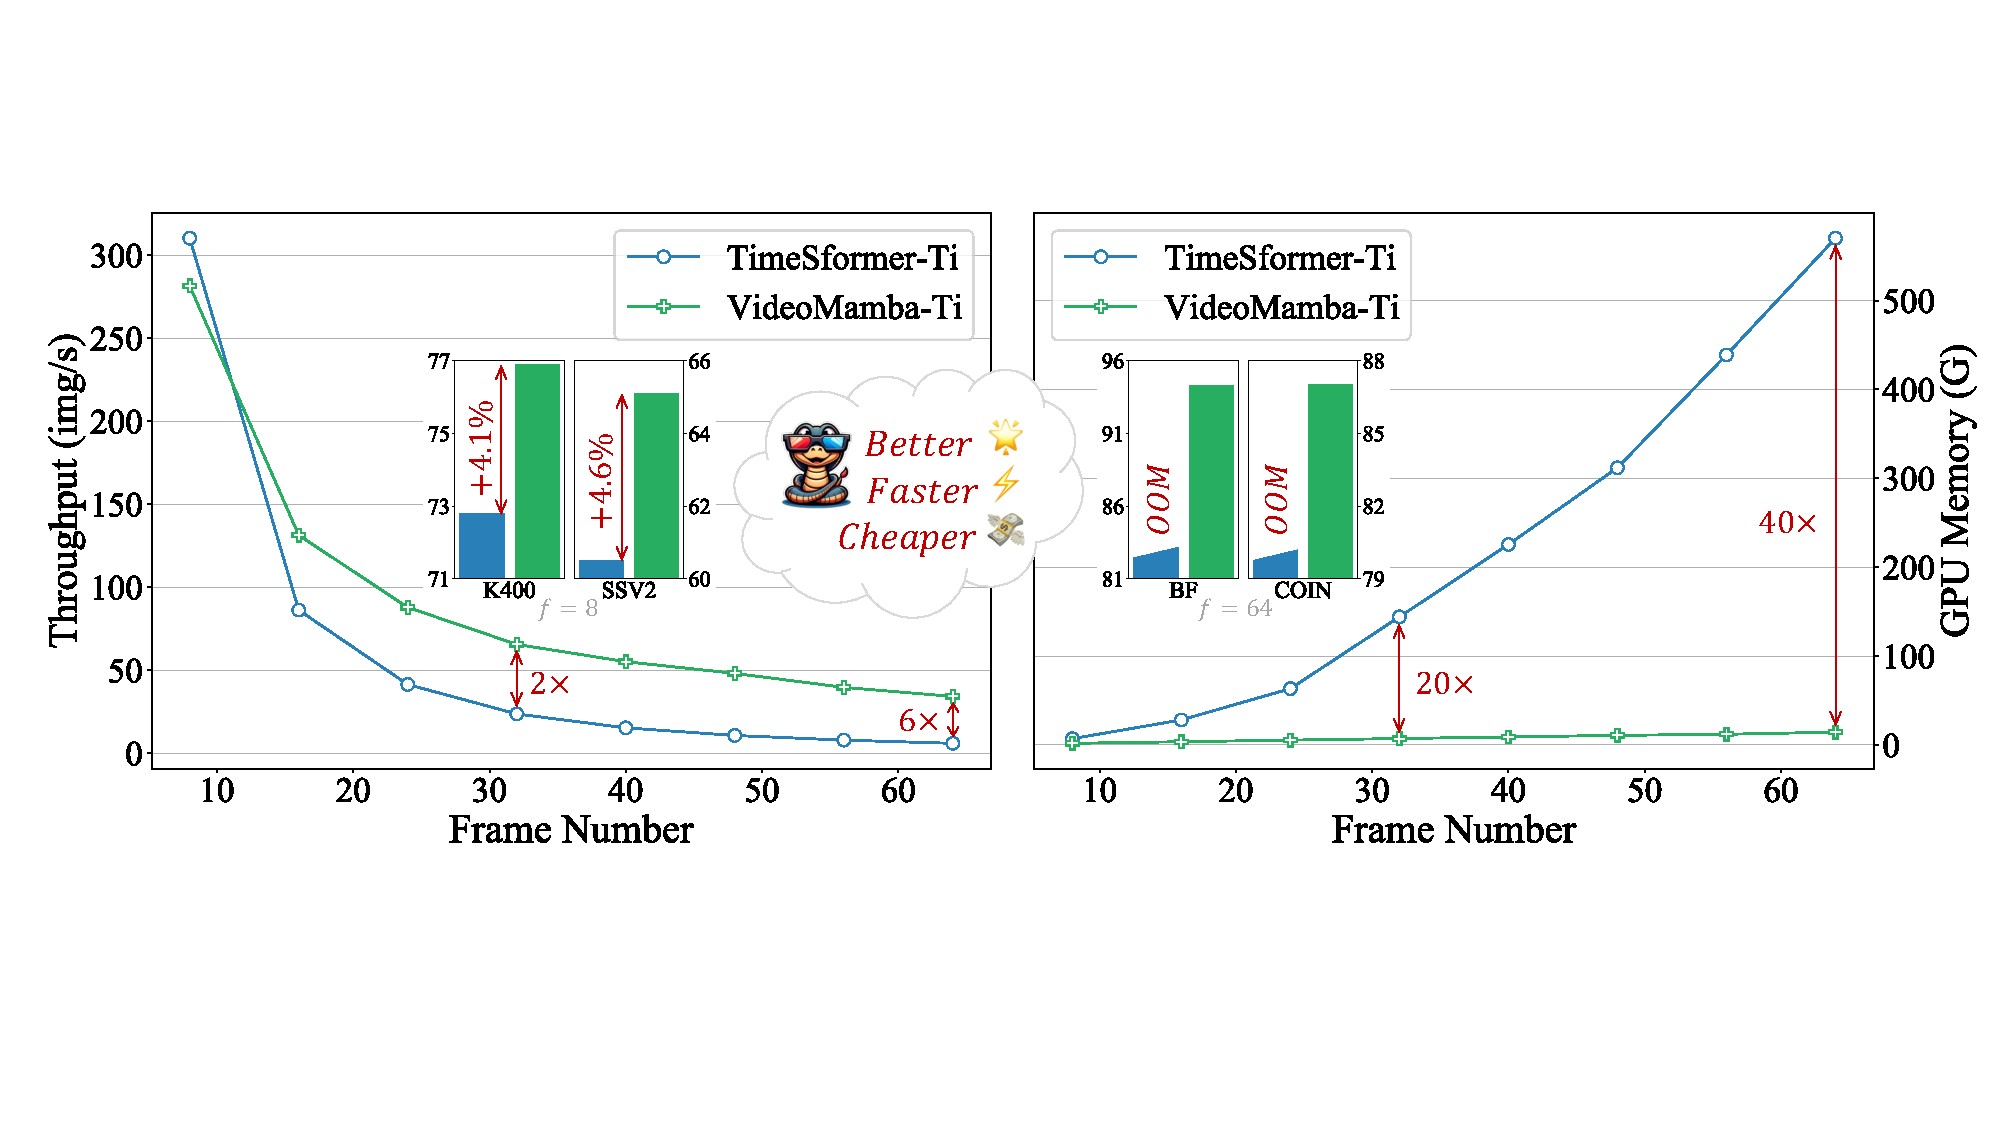
\includegraphics[width=1.0\textwidth]{figs/comparison_memory_speed.pdf}
    \vspace{-0.6cm}
    \caption{\textbf{Comparisons of throughput and memory.}
    The TimeSformer-Ti~\cite{timesformer} is built based on DeiT-Ti~\cite{deit} with joint spatiotemporal attention.
    All the input frames are sized to 224$\times$224.
    The testing is conducted on an NVIDIA A100-80G GPU, utilizing PyTorch 2.1 and CUDA 11.8, with a batch size of 128.
    Our \ModelName\  is \textbf{\textit{better, faster and cheaper}} for both short-term and long-term video understanding.
    } 
    \label{fig:comparison_memory_speed}
    \vspace{-0.3cm}
\end{figure}

The emergence of low-cost operators such as S4~\cite{ssms4}, RWKV~\cite{rwkv}, and RetNet~\cite{retnet} in the NLP domain, 
has carved a novel pathway for the vision model. 
Mamba~\cite{gu2023mamba} stands out with its selective state space model (SSM), 
striking a balance between maintaining linear complexity and facilitating long-term dynamic modeling. 
This innovation has spurred its adoption in vision tasks, 
as evidenced by Vision Mamba~\cite{vim} and VMamba~\cite{vmamba}, 
which leverage multi-directional SSMs for enhanced 2D image processing.
These models rival attention-based architectures in performance while offering a significant reduction in memory usage. 
Given the inherently longer sequences produced by video,
a natural question arises:
\textbf{\textit{Can Mamba work well for video understanding?}}

Inspired by this, 
we introduce \ModelName, 
a purely SSM-based model tailored for video understanding. 
\ModelName\ harmoniously merges the strengths of convolution and attention in vanilla ViT~\cite{vit} style.
It offers a linear-complexity method for dynamic spatiotemporal context modeling, 
ideal for high-resolution long videos. 
The related evaluation focuses on \ModelName's four key abilities:

\textbf{(1) \textit{Scalability in the Visual Domain}:} 
We examine \ModelName's scalability and find that, while the pure Mamba model tends to overfit as it scales, 
our introduction of a simple yet effective self-distillation strategy allows \ModelName\ to achieve remarkable performance enhancements as the model and input sizes increase,
without the need for large-scale dataset pretraining.

\textbf{(2) \textit{Sensitivity for Short-term Action Recognition}:} 
Our analysis extends to assessing \ModelName's capability to accurately distinguish short-term actions,
especially those with fine-grained motion differences, 
\textit{e.g.}, 
opening and closing. 
The findings reveal \ModelName's superior performance over existing attention-based models~\cite{timesformer,vivit,video_swin}.
More importantly,
it is also suitable for masked modeling,
which further enhances its temporal sensitivity. 

\textbf{(3) \textit{Superiority in Long-term Video Understanding}:} 
We then assess \ModelName's prowess in interpreting long videos.
It showcases remarkable superiority over conventional feature-based methods~\cite{vis4mer,distant} through end-to-end training. 
% even with a smaller model size
Notably, 
\ModelName\ operates 6$\times$ faster than TimeSformer~\cite{timesformer} and demands 40$\times$ less GPU memory for 64-frame videos (see Fig. \ref{fig:comparison_memory_speed}).

\textbf{(4) \textit{Compatibility with Other Modalities}:} 
Lastly, 
we assess \ModelName's adaptability with other modalities. 
Results in video-text retrievals show its improved performance than ViT, 
particularly in long videos with complex scenarios.
This underscores its robustness and multi-modal integration capacity.

In conclusion, 
our in-depth experiments reveal \ModelName's immense potential in understanding both short-term (K400~\cite{k400} and SthSthV2~\cite{sth}) and long-term (Breakfast~\cite{breakfast}, COIN~\cite{coin}, and LVU~\cite{lvu}) video contents. 
Given its efficiency and effectiveness, 
\ModelName\ is poised to become a cornerstone in the realm of long-video comprehension.
All the code and models are open-sourced to foster future research endeavors.